\documentclass[aspectratio=169,10pt]{beamer}

\usepackage[T1]{fontenc}
\usepackage[utf8]{inputenc}
\usepackage{lmodern}
\usepackage{graphicx}
\usepackage{booktabs}
\usepackage{array}
\usepackage{xcolor}

\usetheme{Boadilla}
\usecolortheme{seahorse}
\setbeamertemplate{navigation symbols}{}
\setbeamertemplate{footline}[frame number]
\setbeamertemplate{itemize items}[circle]

\graphicspath{{../../results/}{../../specification/}{../img/}}

\definecolor{deepsea}{RGB}{18,76,91}
\definecolor{harbor}{RGB}{230,126,34}
\definecolor{softgray}{RGB}{245,247,249}

\setbeamercolor{title}{fg=deepsea}
\setbeamercolor{frametitle}{fg=deepsea}
\setbeamercolor{structure}{fg=deepsea}
\setbeamercolor{block title}{bg=deepsea,fg=white}
\setbeamercolor{block body}{bg=softgray,fg=black}

\newcommand{\kn}{\ensuremath{\,\mathrm{kn}}}
\newcommand{\kw}{\ensuremath{\,\mathrm{kW}}}
\newcommand{\co}{CO$_2$}

\title[Maritime Performance Analytics]{Wind-Assisted Propulsion on North Sea Routes}
\subtitle{Maritime performance analytics for Flettner rotors}
\author[A. Klos et al.]{
Aleksandra K\l{}os \and Olga Grigorieva \and Elen Mouradian \and Bartosz Maj \and Hubert Jaczy\'nski
}
\institute{DataWaves Innovation Laboratory}
\date{May 2026}

\begin{document}

\begin{frame}
    \titlepage
\end{frame}

\begin{frame}{Project Question}
    \begin{columns}[T,onlytextwidth]
        \begin{column}{0.52\textwidth}
            \begin{block}{Aim}
                Estimate how weather and Flettner rotor assistance affect vessel speed, fuel use, emissions, and route choice.
            \end{block}
            \vspace{0.25cm}
            \begin{itemize}
                \item Combine AIS trajectories with wind, waves, and currents.
                \item Predict speed under metocean conditions.
                \item Convert rotor assistance into speed, fuel, and \co{} effects.
                \item Extend the analysis toward uncertainty-aware routing.
            \end{itemize}
        \end{column}
        \begin{column}{0.44\textwidth}
            \centering
            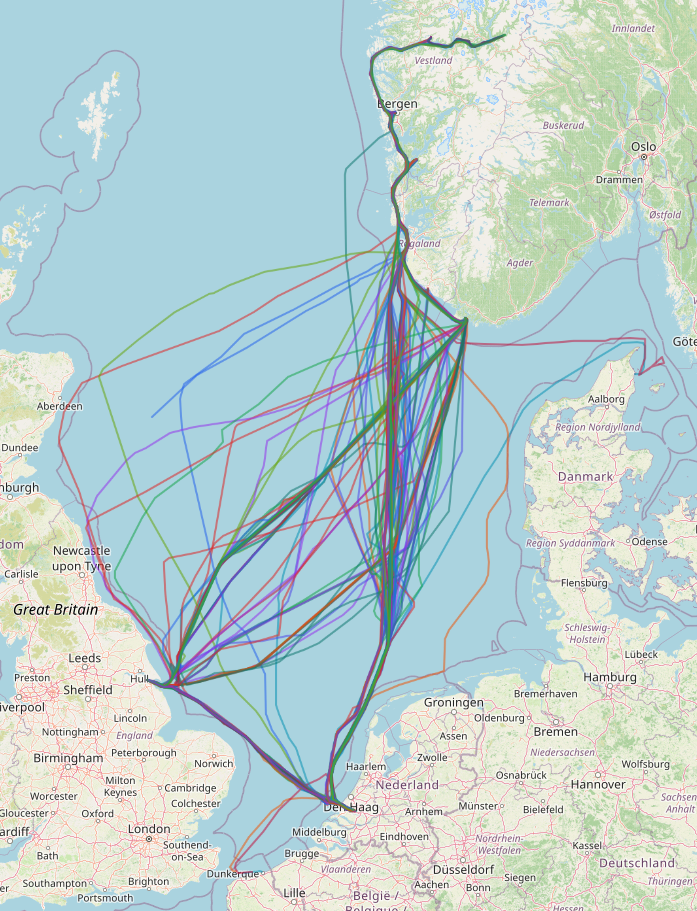
\includegraphics[width=\linewidth,height=0.68\textheight,keepaspectratio]{all_trajectories_osm.png}
        \end{column}
    \end{columns}
\end{frame}

\begin{frame}{Data And Feature Pipeline}
    \begin{columns}[T,onlytextwidth]
        \begin{column}{0.50\textwidth}
            \begin{itemize}
                \item 125,160 AIS-metocean observations.
                \item 528 voyages from 2023-02-02 to 2026-02-02.
                \item Chronological voyage split: 422 train voyages, 106 test voyages.
                \item Features: speed, course, wind angle, wave height, current, and trajectory context.
            \end{itemize}
        \end{column}
        \begin{column}{0.46\textwidth}
            \begin{block}{Why the split matters}
                Observations from one voyage stay on one side of the train/test boundary, reducing temporal and trajectory leakage.
            \end{block}
            \vspace{0.25cm}
            \begin{block}{Core target}
                Speed over ground (SOG), measured in knots.
            \end{block}
        \end{column}
    \end{columns}
\end{frame}

\begin{frame}{Speed Model Results}
    \centering
    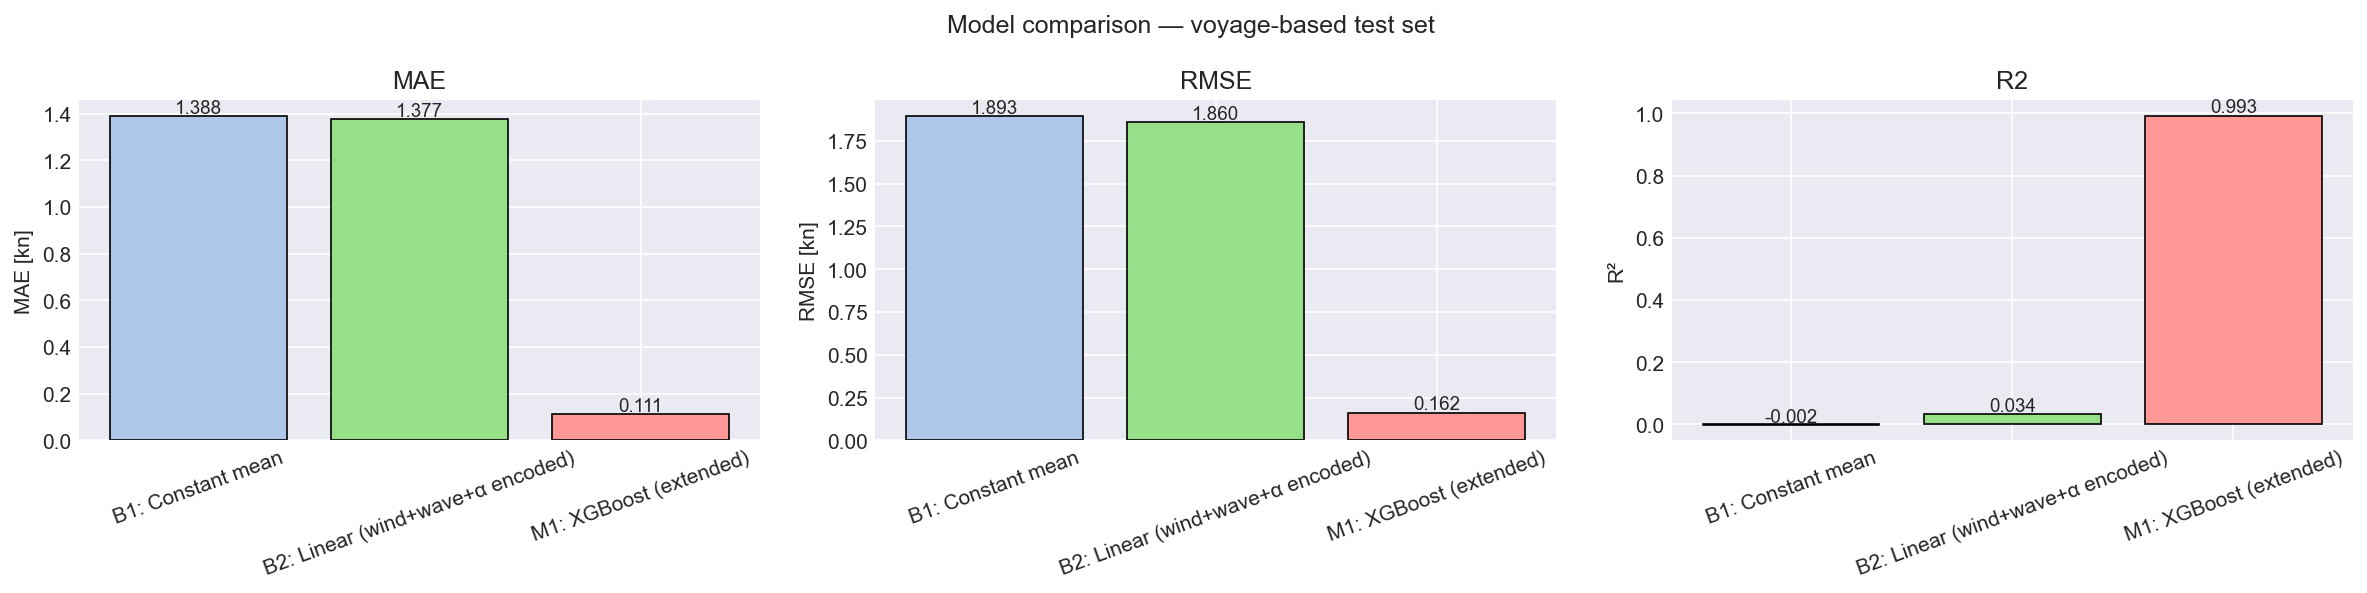
\includegraphics[width=1\linewidth,height=0.76\textheight,keepaspectratio]{model_comparison.png}
\end{frame}

\begin{frame}{Speed Model Interpretation}
    \begin{block}{Main result}
        The strongest model is the lagged nowcast XGBoost model, which uses recent speed and apparent wind context.
    \end{block}
    \vspace{0.25cm}
    \begin{columns}[T,onlytextwidth]
        \begin{column}{0.48\textwidth}
            \begin{itemize}
                \item Test MAE: 0.406\kn{}.
                \item Test RMSE: 0.758\kn{}.
                \item Test $R^2$: 0.839.
            \end{itemize}
        \end{column}
        \begin{column}{0.48\textwidth}
            \begin{itemize}
                \item 91.7\% within $\pm$1\kn{}.
                \item Weather-only modelling is more useful for interpretation than pure prediction.
                \item Baselines remain important sanity checks.
            \end{itemize}
        \end{column}
    \end{columns}
\end{frame}

\begin{frame}{Rotor Opportunity Scenario}
    \begin{columns}[T,onlytextwidth]
        \begin{column}{0.50\textwidth}
            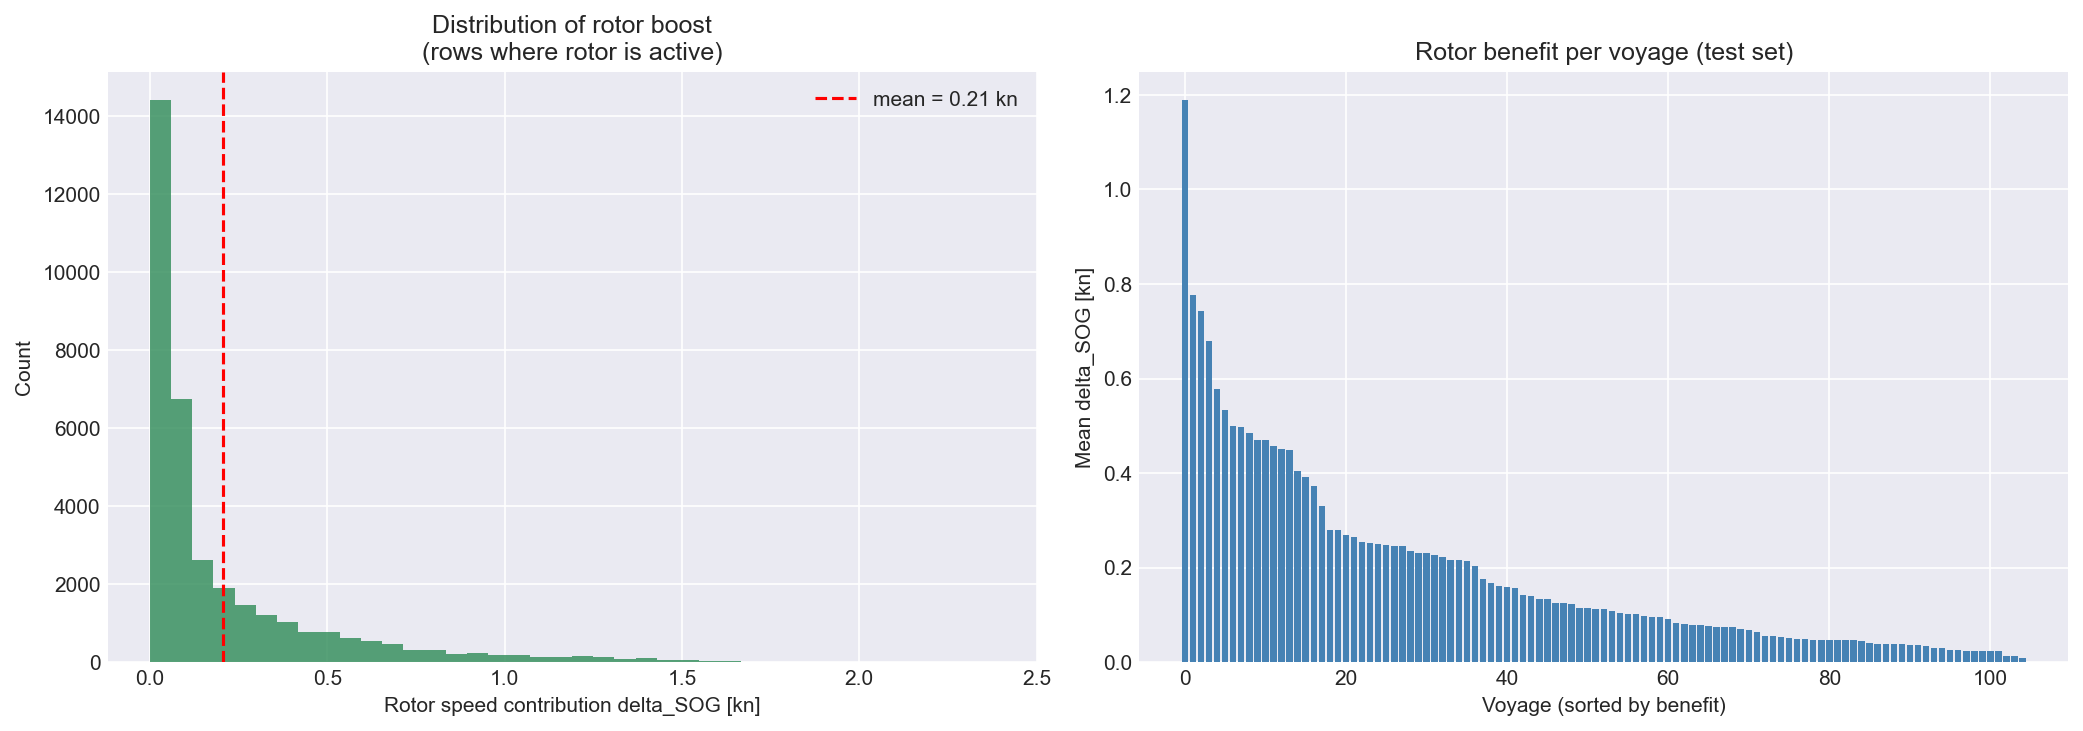
\includegraphics[width=\linewidth]{rotor_scenario.png}
        \end{column}
        \begin{column}{0.46\textwidth}
            \begin{itemize}
                \item Rotor power is estimated from the provided polar diagram.
                \item Scenario conversion: 200\kw{} $\approx$ 1\kn{} near the operating point.
                \item Rotor active in 98.1\% of held-out observations.
                \item Mean speed contribution: 0.202\kn{} overall.
                \item Weather-window coverage: 76.0\% $\rightarrow$ 77.5\%.
                \item Dataset estimate: 112.2 t fuel and 349.4 t \co{} avoided.
            \end{itemize}
        \end{column}
    \end{columns}
\end{frame}

\begin{frame}{Monte Carlo Routing Extension}
    \begin{columns}[T,onlytextwidth]
        \begin{column}{0.55\textwidth}
            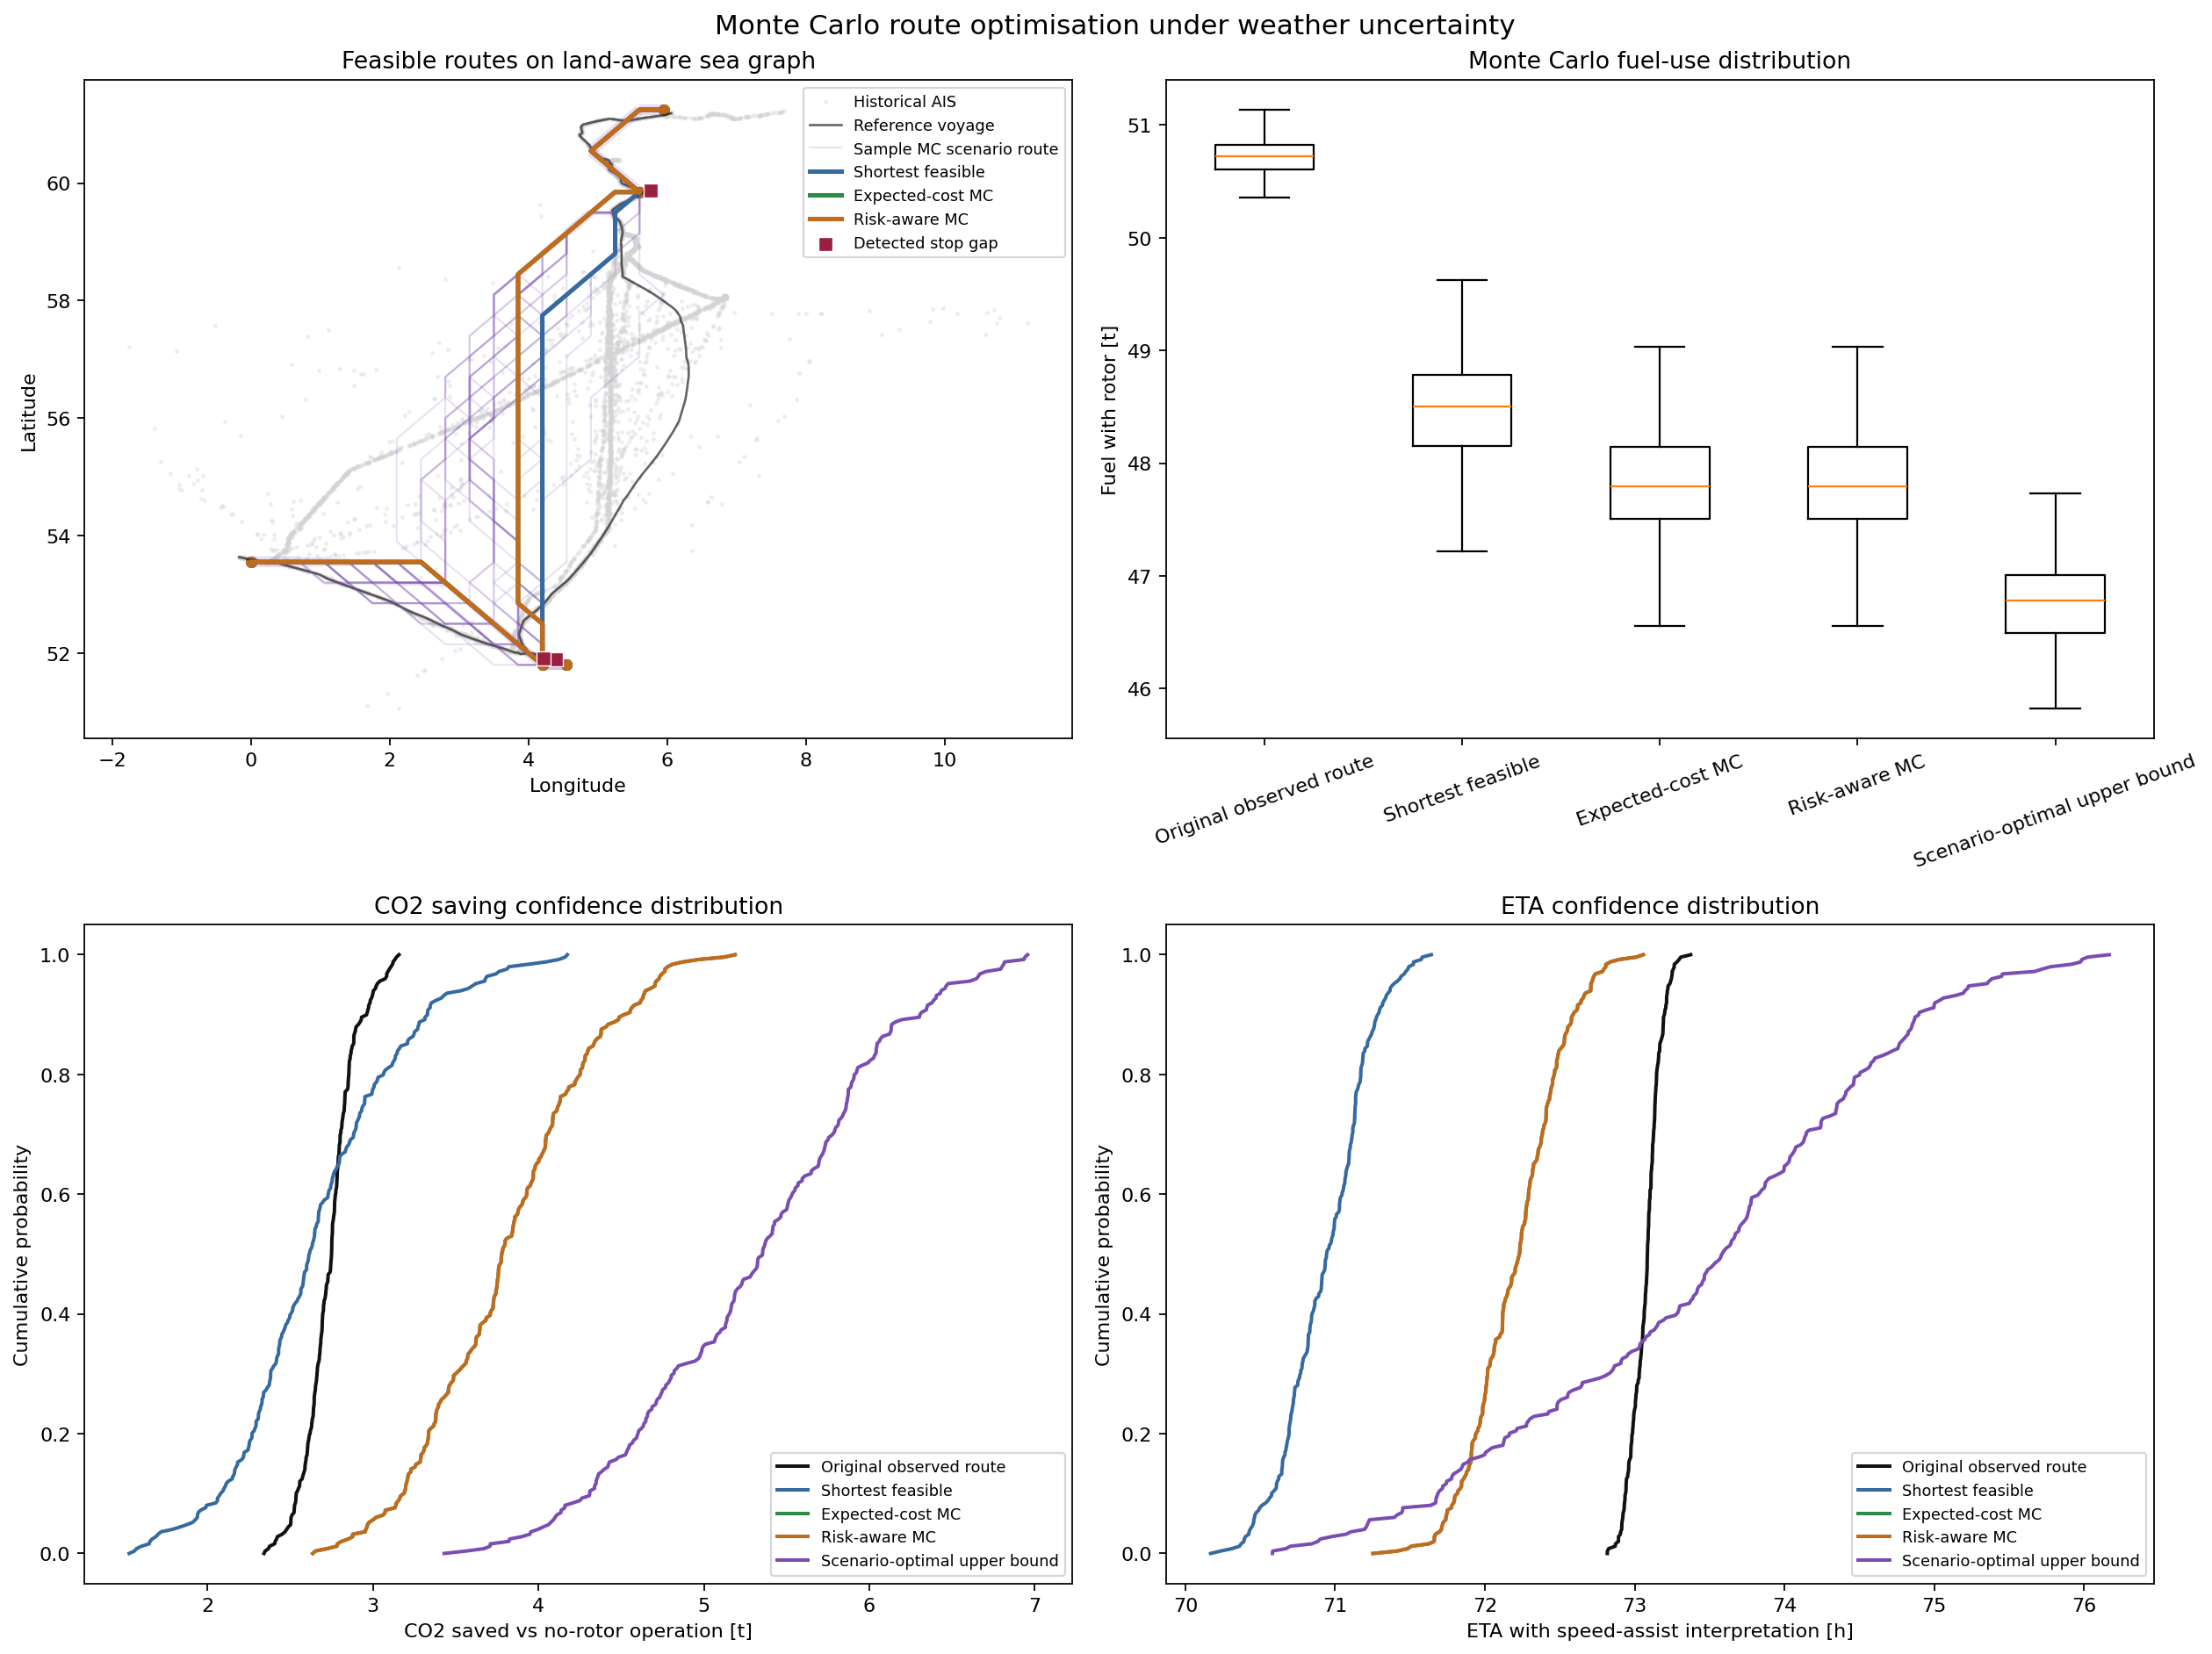
\includegraphics[width=\linewidth]{monte_carlo_routing.png}
        \end{column}
        \begin{column}{0.41\textwidth}
            \begin{itemize}
                \item Keeps the detected itinerary: 4 sailing legs and 3 stop gaps.
                \item Uses a land-aware graph, with AIS corridor overrides near ports.
                \item Samples multiple weather and rotor scenarios, not only one optimal path.
            \end{itemize}
            \vspace{0.15cm}
            \scriptsize
            \begin{tabular}{lrrrr}
                \toprule
                Route & nm & fuel & saved & $P$ \\
                \midrule
                Original & 863.6 & 50.72 & 0.88 & -- \\
                Shortest & 834.1 & 48.47 & 0.86 & 0.00 \\
                MC cost & 847.9 & 47.81 & 1.22 & 0.86 \\
                Scenario best & 860.9 & 46.75 & 1.70 & 1.00 \\
                \bottomrule
            \end{tabular}
            \vspace{0.05cm}

            \scriptsize Fuel and saved fuel are tonnes; $P$ is probability of beating the shortest feasible route on fuel.
        \end{column}
    \end{columns}
\end{frame}

\begin{frame}{Takeaways And Next Steps}
    \begin{block}{What we have now}
        \begin{itemize}
            \item A leakage-aware modelling pipeline.
            \item A transparent rotor what-if scenario.
            \item Fuel and \co{} estimates over voyages.
            \item A multi-leg, land-aware Monte Carlo routing prototype.
            \item Route comparisons with uncertainty, confidence intervals, and scenario paths.
        \end{itemize}
    \end{block}
\end{frame}

\begin{frame}[plain]
    \centering
    \vfill
    {\Huge\bfseries\color{deepsea} See you at the conference!}
    \vspace{0.5cm}

    {\large DataWaves Innovation Laboratory}
    \vfill
\end{frame}

\end{document}
